\documentclass[conference]{IEEEtran}
\IEEEoverridecommandlockouts

\usepackage{cite}
\usepackage{amsmath,amssymb,amsfonts}
\usepackage{algorithmic}
\usepackage{graphicx}
\usepackage{textcomp}
\usepackage{xcolor}
\usepackage{url}
\def\BibTeX{{\rm B\kern-.05em{\sc i\kern-.025em b}\kern-.08em
    T\kern-.1667em\lower.7ex\hbox{E}\kern-.125emX}}
\begin{document}

\title{\title{A Polymorphic Homework System for Supporting Educational Management and Personalized Learning}}

\author{
\IEEEauthorblockN{ChengJun He\textsuperscript{1}, Xinguo Yu\textsuperscript{1}, Hao Meng\textsuperscript{1}}
\IEEEauthorblockA{\textsuperscript{1}Faculty of Artificial Intelligence in Education, Central China Normal University, Wuhan, China\\
Email: 1832094726@mails.ccnu.edu.cn, xgyu@ccnu.edu.cn, menghao@mails.ccnu.edu.cn}
}

\maketitle
\begin{abstract}
Traditional homework systems often fail to provide adequate support for diverse learning environments and individual student needs, leading to reduced engagement and suboptimal educational outcomes. More critically, these systems lack structured approaches to educational management, making it difficult for educators to effectively track, analyze, and support student learning at scale. This paper presents a comprehensive homework system that addresses these limitations by introducing a novel structured personalized learning framework composed of the Adaptive Learning Profile (ALP) and the Learning Evolution Graph (LEG). At the core of this innovation is the system’s ability to generate structured learning profiles and management data as natural outputs of personalized learning activities, creating a robust foundation for educational management. Unlike conventional systems that isolate learning tools from management functions, our polymorphic design integrates personalized learning delivery with structured data generation—enabling seamless educational management through standardized learning profiles, progress tracking structures, and automated reporting mechanisms. The ALP and LEG frameworks capture and organize learning behaviors, knowledge trajectories, and evolutionary patterns of individual learning processes, while the system’s multi-dimensional adaptation across devices, user roles, and learning contexts generates comprehensive management outputs to facilitate effective educational oversight.
\end{abstract}

\begin{IEEEkeywords}
\begin{IEEEkeywords}
adaptive learning profile, learning evolution graph, personalized learning frameworks, educational management, structured learning systems, polymorphic homework system
\end{IEEEkeywords}

\section{Introduction}

Educational resources in the digital age have expanded rapidly, creating both opportunities and challenges for students. Modern learners are required to navigate multiple platforms daily \cite{author2020educational}, leading to cognitive overload and reduced learning efficiency \cite{sweller2024cognitive}. This abundance of resources introduces information overload, making it difficult for students to identify relevant content for their learning needs \cite{paas2025measurement}.

Homework serves as a cornerstone of K-12 mathematics education, providing a mechanism for students to consolidate knowledge and practice problem-solving skills \cite{cooper2024homework}. However, traditional homework paradigms lack the dynamic adaptability necessary to cater to diverse learning styles and individual student needs \cite{deci2025intrinsic}. When difficulties are encountered, the absence of immediate assistance leads to unproductive struggle and reduced motivation \cite{ryan2024self}.

The fundamental challenge lies in creating effective connections between personalized learning enhancement and educational management support within homework systems. Traditional approaches treat these as separate concerns, requiring educators to choose between systems optimized for individual learning experiences and those designed for administrative oversight. This paper presents a polymorphic homework system that addresses this connection challenge through an innovative dual-support architecture that simultaneously enhances personalized learning and generates comprehensive educational management data.

The core innovation lies in designing connection mechanisms that enable homework activities to naturally produce both immediate personalized learning benefits and structured educational management insights. Through the integration of Adaptive Learning Profile (ALP) and Learning Evolution Graph (LEG) frameworks within the homework workflow, our system demonstrates how individual learning enhancement and educational oversight can be achieved synergistically rather than competitively \cite{brusilovsky2024adaptive}. The ALP framework captures real-time learning behaviors and preferences during homework completion, while the LEG framework traces learning evolution patterns that inform both personalized interventions and management decisions \cite{ricci2025introduction}.

Unlike conventional systems that require separate data collection mechanisms for learning support and management functions, our polymorphic homework system embeds connection points throughout the homework workflow that seamlessly generate dual-value outputs. This approach transforms homework completion from a simple assignment submission process into a rich data generation activity that supports both student learning optimization and educational management decision-making.

The proposed homework system implements connection mechanisms through strategic integration points embedded within the existing homework workflow. Rather than requiring separate data collection systems, our approach leverages natural homework activities as connection points that simultaneously generate personalized learning enhancements and educational management insights \cite{zhang2025deep}. The system architecture demonstrates how homework completion activities can be transformed into rich data generation processes through three key connection layers: behavioral data collection during homework interactions, real-time framework processing that generates both ALP profiles and LEG trajectories, and dual-output generation that provides immediate learning support while building comprehensive management datasets \cite{sharples2024mobile}. This connection-oriented design ensures that every homework activity contributes to both individual learning optimization and systematic educational oversight without requiring additional effort from students or educators.

This paper presents a comprehensive exposition of our polymorphic homework system, demonstrating how structured learning frameworks can simultaneously enhance student learning experiences and generate comprehensive educational management data \cite{lu2025recommender}. The system architecture, structured profile generation mechanisms, management data synthesis processes, and practical implementation are detailed to show how personalized learning methodologies can naturally produce the structured outputs necessary for effective educational management \cite{koedinger2024learning}. The key contribution lies in proving that student-centered design and educational management efficiency are not competing objectives, but can be achieved synergistically through appropriate system architecture and data structure design.



\section{Polymorphic Homework System for Dual Support Goals}

This section presents the core methodology of our polymorphic student-side homework system, focusing on how the system achieves adaptive behavior across different devices, user roles, and learning scenarios while maintaining consistent functionality and user experience.

\subsection{Polymorphic System Design}

The polymorphic nature of our system is achieved through a context-aware architecture that dynamically adapts its interface, functionality, and content delivery based on three key dimensions: device modality, user role, and learning context. The system maintains a unified core logic while presenting different user experiences optimized for each specific context.

The system automatically detects the accessing device type and adapts its interface accordingly. For touch devices such as tablets and smartphones, the interface prioritizes larger touch targets, gesture-based navigation, and touch-optimized mathematical input. When accessed through keyboard-based devices like PCs and laptops, the system emphasizes keyboard shortcuts, precise cursor control, and high-resolution display optimization. For voice-enabled devices including educational robots, the interface provides phonetic descriptions and voice command support to accommodate different interaction modalities.

Different interfaces are presented based on user roles to ensure appropriate functionality for each user type. Students interact with a focused homework completion interface that provides intelligent assistance features and real-time guidance. Teachers access a comprehensive dashboard that enables assignment creation, progress monitoring, and detailed student analytics. Parents view a simplified portal that shows homework progress and highlights areas where additional attention may be needed, facilitating family engagement in the learning process.

The system also adapts its behavior based on the current learning scenario to provide contextually appropriate support. During individual study sessions, detailed explanations and step-by-step guidance are provided to support self-directed learning. In timed assessments, the interface emphasizes efficiency and provides quick access to essential tools to minimize distractions. For collaborative learning sessions, the system facilitates peer interaction and group problem-solving through shared workspaces and communication tools.

\subsection{Dual-Support Architecture Design}

The core challenge in connecting personalized learning and educational management lies in designing system architecture that can simultaneously optimize individual learning experiences while generating systematic management data. Traditional homework systems require educators to choose between student-centered learning tools and management-oriented administrative systems. Our polymorphic homework system addresses this challenge through a dual-support architecture that treats connection as a fundamental design principle rather than an afterthought.

The dual-support architecture operates on three key principles: seamless data flow integration, where homework activities naturally generate both learning enhancement and management insights; real-time dual processing, where student interactions simultaneously trigger personalized recommendations and management data updates; and unified value generation, where every system component contributes to both individual learning optimization and educational oversight. This architecture ensures that the system's primary function of supporting student learning is enhanced rather than compromised by management data generation requirements.

The architecture implements connection mechanisms through strategic integration points embedded within the homework workflow. These integration points capture learning behaviors during natural homework activities, process this data through both personalized learning algorithms and management analytics engines, and generate outputs that serve both immediate student needs and long-term educational planning. This approach transforms homework completion from a simple task submission process into a rich data generation activity that benefits all stakeholders in the educational ecosystem.

\subsection{Adaptive Learning Profile (ALP) Framework}

The Adaptive Learning Profile framework serves as a critical connection component that transforms individual homework activities into structured learning insights while simultaneously generating educational management data. Unlike traditional student records that capture only final outcomes, ALP creates dynamic profiles that evolve with each homework interaction, providing real-time value for both personalized learning enhancement and systematic educational oversight.

The ALP framework operates as a connection mechanism through four integrated dimensions that serve dual purposes. Learning behavior patterns capture how students approach homework problems, including problem-solving strategies, time allocation patterns, help-seeking behaviors, and error correction methods. This behavioral analysis enables immediate personalized recommendations for individual students while generating aggregate behavioral insights that inform classroom-level instructional decisions and curriculum optimization.

Knowledge mastery mapping provides detailed understanding of concept comprehension across different mathematical domains through skill proficiency matrices, knowledge gap identification, and learning prerequisite tracking. This mapping creates comprehensive individual learning profiles that drive personalized content recommendations while simultaneously generating class-wide mastery analytics that support educational planning and intervention strategies.

Personalized learning pathways emerge from the analysis of individual learning patterns, generating optimal learning sequences, difficulty progression curves, and motivation trigger points tailored to each student's characteristics. These pathways enable targeted individual support while contributing to broader understanding of effective learning sequences that inform curriculum design and instructional methodology.

Performance analytics synthesize learning data into actionable insights through learning efficiency metrics, engagement level tracking, and achievement pattern recognition. This analytical layer transforms raw homework interaction data into structured profiles that support immediate personalized interventions while generating systematic performance data that facilitates educational management decision-making and quality assurance processes.

\begin{figure}[htbp]
\centerline{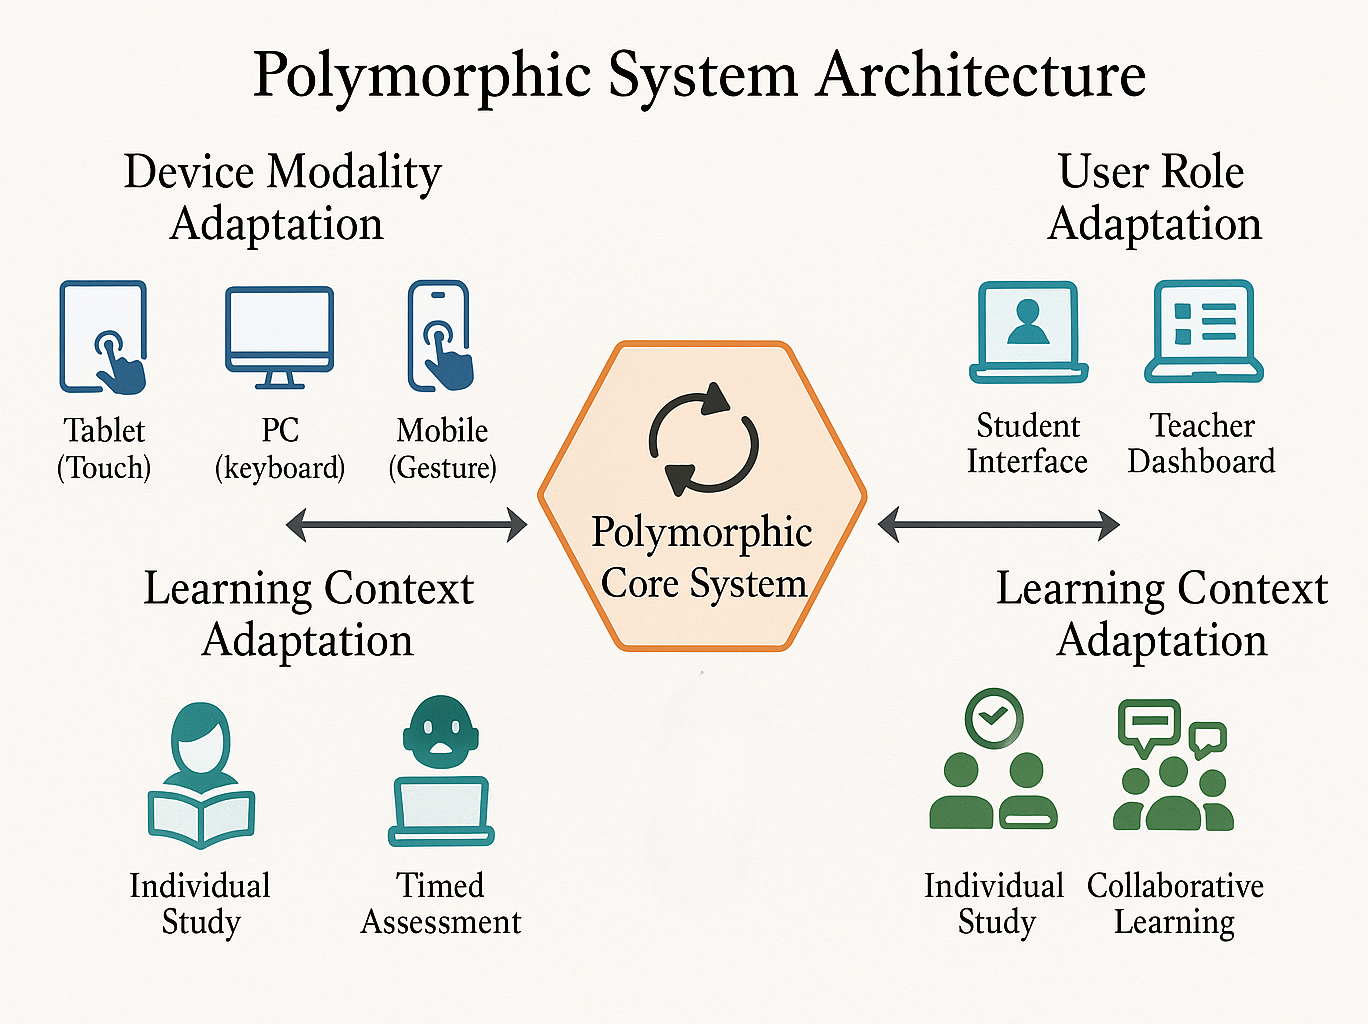
\includegraphics[width=\columnwidth]{1.png}}
\caption{Adaptive Learning Profile (ALP) Framework Structure showing the four primary dimensions: learning behavior patterns, knowledge mastery mapping, personalized learning pathways, and performance analytics with their interconnected data flows.}
\label{fig:alp_framework}
\end{figure}

\subsection{Learning Evolution Graph (LEG) Framework}

The Learning Evolution Graph framework functions as a temporal connection mechanism that traces individual learning development while generating predictive insights for educational management. Unlike static assessment records, LEG creates dynamic learning trajectories that evolve with each homework session, providing both immediate learning support and long-term educational planning data.

The LEG framework structures learning evolution through four interconnected components that serve dual connection purposes. Temporal learning nodes capture key moments in homework completion processes, including knowledge acquisition points, skill development milestones, difficulty breakthrough moments, and learning strategy adaptations. These nodes create individual learning timelines that inform personalized intervention timing while generating aggregate learning progression data that supports curriculum pacing and instructional planning decisions.

Learning relationship edges connect temporal nodes through prerequisite dependencies, concept associations, skill transfer connections, and learning reinforcement links. This network structure reveals how individual learning in one area influences development in others, enabling personalized learning path optimization while providing systematic insights into knowledge interconnections that inform curriculum design and instructional sequencing.

Evolution trajectories analyze individual learning development patterns through learning path optimization, knowledge network expansion, and adaptive strategy evolution. These trajectories reveal how individual students' learning approaches change over time and identify optimal intervention points for personal support while contributing to broader understanding of effective learning progressions that inform educational methodology and policy development.

Predictive modeling components use historical learning patterns to forecast individual future learning needs, identify potential difficulty areas, and suggest optimal intervention points. This predictive capability enables proactive personalized educational support while generating systematic forecasting data that supports resource allocation, intervention planning, and educational quality assurance at institutional levels.

\begin{figure}[htbp]
\centerline{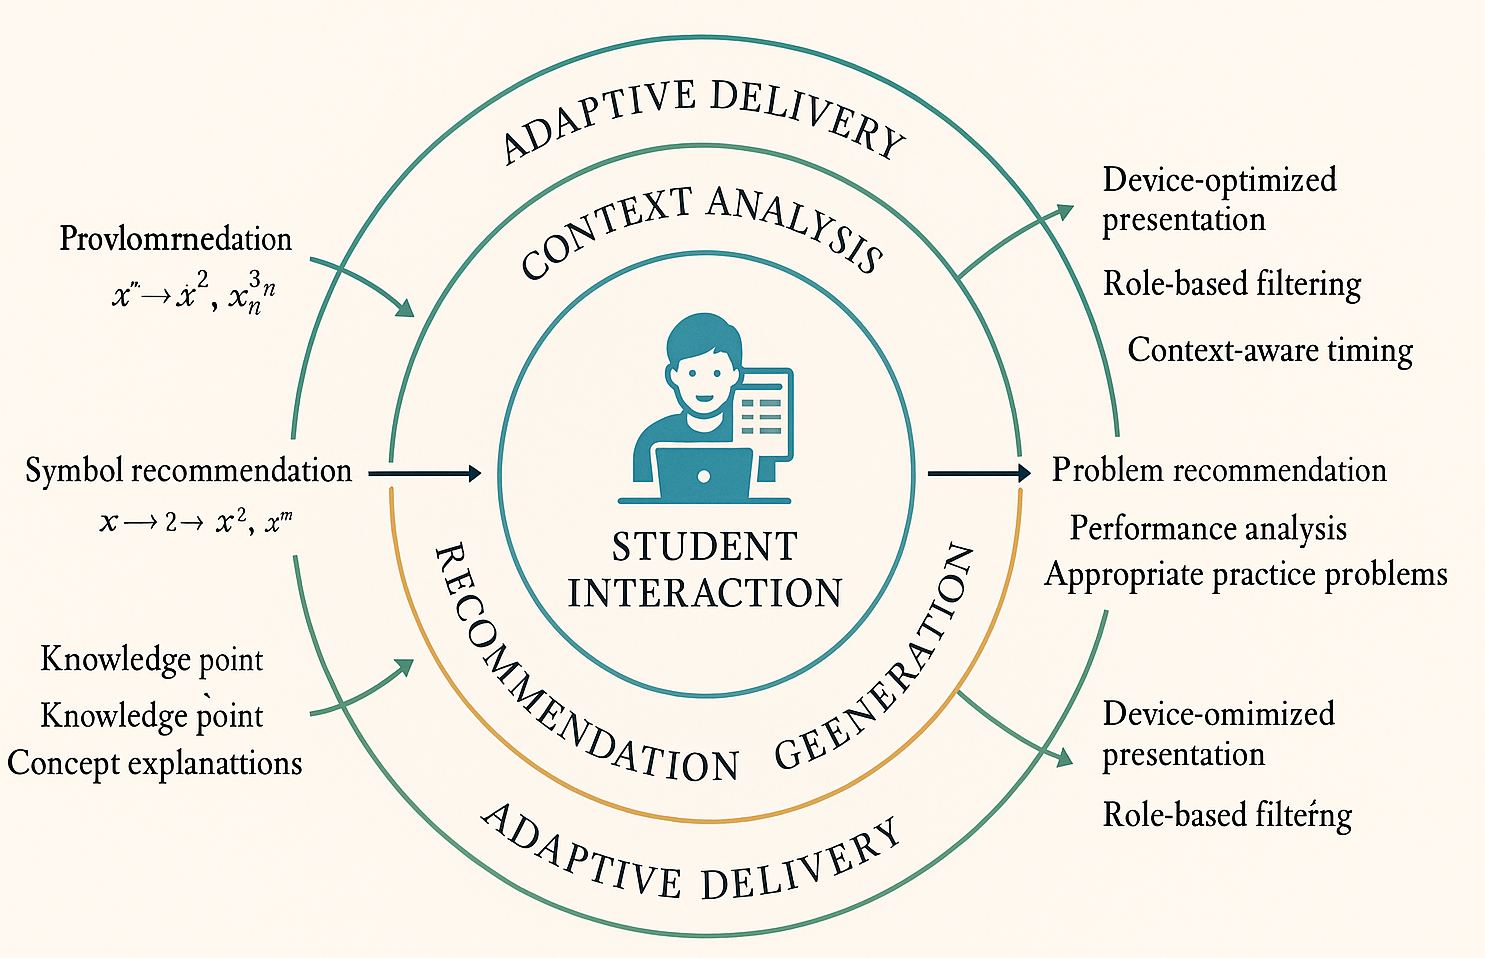
\includegraphics[width=\columnwidth]{2.png}}
\caption{Learning Evolution Graph (LEG) Framework Structure illustrating temporal learning nodes, relationship edges, evolution trajectories, and predictive modeling components with time-based learning development visualization.}
\label{fig:leg_framework}
\end{figure}

\subsection{Connection Point Design and Implementation}

The effectiveness of our dual-support architecture depends on strategically designed connection points embedded throughout the homework workflow that capture learning data without disrupting the natural homework completion process. These connection points transform routine homework activities into rich data generation opportunities that simultaneously enhance individual learning and support educational management.

Connection points are implemented at three critical levels within the homework system architecture. Interface-level connection points capture user interaction patterns during homework completion, including click sequences, time allocation patterns, help-seeking behaviors, and error correction strategies. These interactions are processed in real-time to generate immediate personalized recommendations while contributing to comprehensive behavioral analytics that inform instructional design and curriculum optimization decisions.

Process-level connection points monitor learning progression during homework completion, tracking knowledge application patterns, problem-solving strategy evolution, and conceptual understanding development. This process monitoring enables dynamic difficulty adjustment and personalized content sequencing for individual students while generating systematic learning progression data that supports educational planning and quality assurance at classroom and institutional levels.

Outcome-level connection points analyze homework completion results to assess learning effectiveness, knowledge retention, and skill development. These analyses drive personalized review recommendations and adaptive learning path adjustments for individual students while producing comprehensive performance analytics that facilitate educational management decision-making and intervention planning.

The connection point architecture ensures seamless data flow between individual learning enhancement and educational management functions. Each homework interaction generates data that is simultaneously processed through personalized learning algorithms and management analytics engines, creating dual-value outputs that serve both immediate student needs and long-term educational planning requirements without requiring additional effort from students or educators.

\begin{figure}[htbp]
\centerline{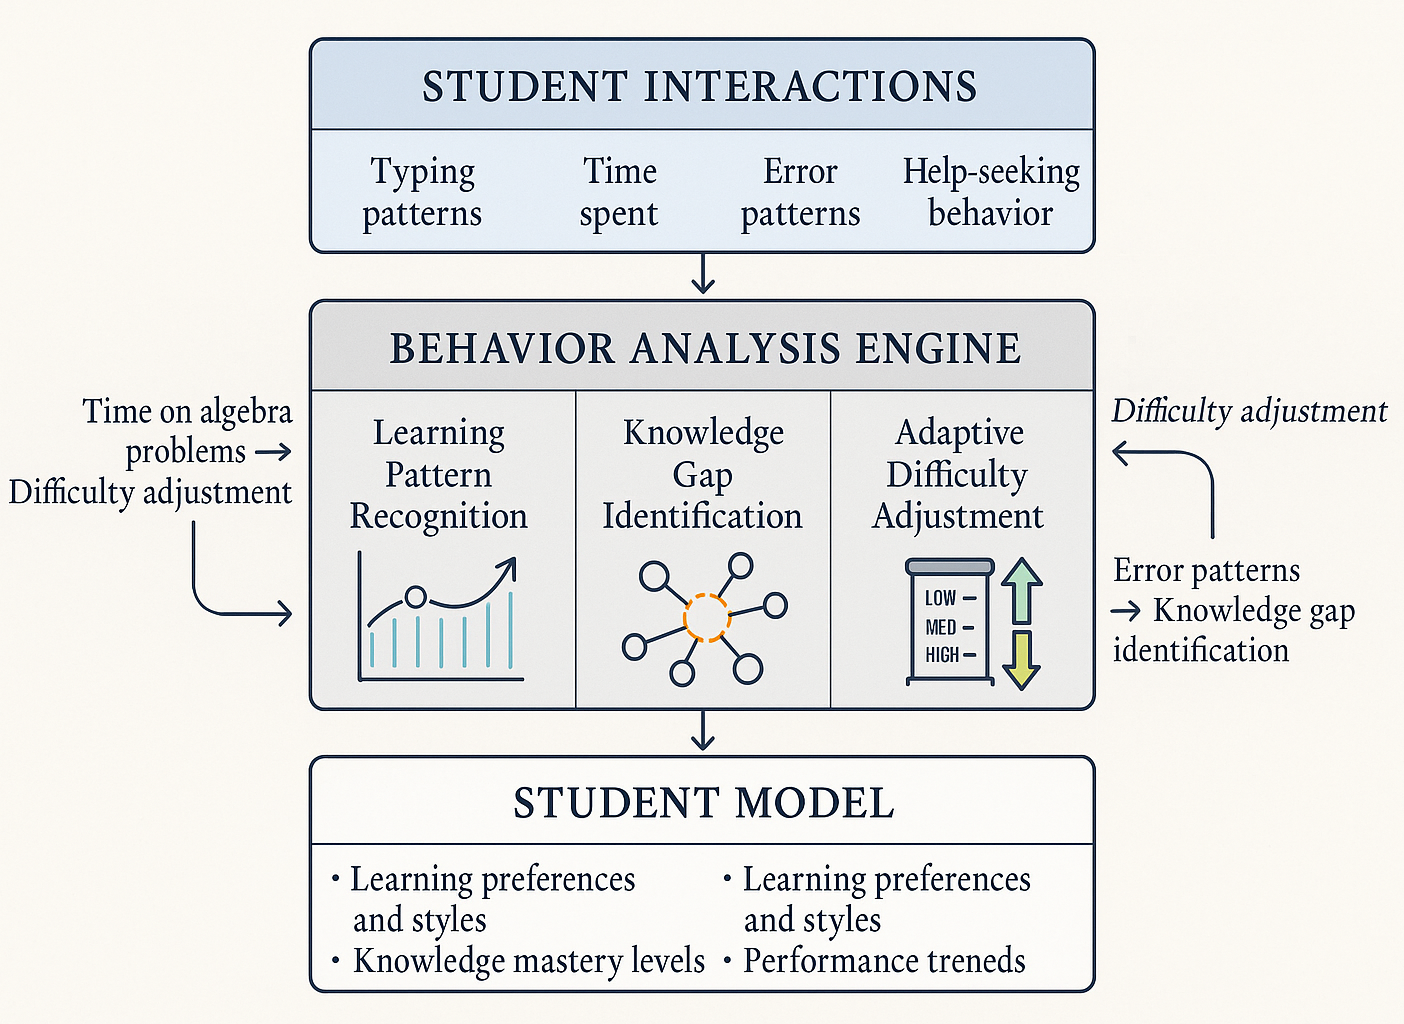
\includegraphics[width=\columnwidth]{3.png}}
\caption{Framework-to-Module Mapping Architecture showing how ALP and LEG backend frameworks drive frontend educational modules including symbol recommendation, homework assignment, knowledge point recommendation, and progress visualization interfaces.}
\label{fig:framework_mapping}
\end{figure}

\subsection{Intelligent Recommendation System}

The core of our system's intelligence lies in its multi-layered recommendation engine that provides contextually appropriate assistance throughout the homework completion process. This engine continuously analyzes student interactions and learning patterns to deliver personalized recommendations that enhance both learning efficiency and engagement.

The mathematical symbol recommendation component analyzes the current mathematical context and predicts the most likely next symbols based on the problem type, current expression, and user's input history. For example, when a student types "x\^{}" in an algebra problem, the system immediately suggests common exponent options ($x^2$, $x^3$, $x^n$) along with other frequently used symbols in similar contexts. The recommendation algorithm considers multiple factors including the current mathematical expression context, problem type and difficulty level, student's previous symbol usage patterns, and common mathematical conventions for the subject area.

When students encounter difficulties during problem-solving, the knowledge point recommendation system identifies knowledge gaps and recommends relevant concepts, formulas, or problem-solving strategies. The recommendation engine analyzes the current problem-solving steps, student's knowledge mastery profile, common misconceptions in the topic area, and optimal learning sequences for concept understanding. This enables the system to provide targeted support that addresses specific learning needs rather than generic assistance.

The problem recommendation system suggests appropriate practice problems that match the student's current learning level and address identified knowledge gaps. Problem selection considers the current topic mastery level, learning progression requirements, student's preferred difficulty range, and available time for practice. This ensures that students receive appropriately challenging problems that support their learning progression without causing frustration or boredom.

\subsection{Student Behavior Modeling for ALP and LEG Generation}

The system's student behavior modeling component serves as the data collection foundation for both ALP and LEG frameworks. This component continuously analyzes student interactions to extract the behavioral patterns and learning trajectories that populate the structured representations used by both frameworks.

The system tracks various aspects of student behavior during homework completion to build comprehensive learning profiles. These include time spent on different problem types, error patterns and correction strategies, symbol and formula usage frequency, problem-solving approach preferences, and help-seeking behavior patterns. By analyzing these behavioral indicators, the system can identify learning preferences and areas where additional support may be beneficial.

Through analysis of homework submissions and interaction patterns, the system identifies concepts that consistently cause difficulties, misconceptions that lead to repeated errors, areas where additional practice is needed, and optimal learning paths for concept mastery. This knowledge gap identification enables the system to provide targeted interventions that address specific learning challenges rather than generic assistance.

The system dynamically adjusts problem difficulty based on multiple factors including student's recent performance trends, time spent on similar problems, error frequency and types, and self-reported confidence levels. This adaptive difficulty adjustment ensures that students are consistently challenged at an appropriate level that promotes learning without causing frustration or disengagement.

\subsection{Cross-Device User Experience}

The system ensures consistent functionality and seamless experience across different devices while optimizing for each device's unique capabilities. This cross-device consistency is achieved through intelligent data management and interface adaptation that maintains user experience quality regardless of the accessing device.

Student progress, preferences, and learning data are automatically synchronized across all devices to ensure continuity in the learning experience. This synchronization includes real-time progress updates, consistent user preferences, seamless device switching, and offline capability with automatic synchronization when connectivity is restored. The system maintains learning context when students switch between devices, preserving current problem-solving states, work-in-progress calculations, recent recommendations and help content, and learning session continuity.

\subsection{Real-Time Feedback and Assistance}

The system provides immediate, contextual assistance throughout the homework completion process, significantly reducing unproductive struggle time and enhancing learning effectiveness. This real-time support system ensures that students receive help when they need it most, preventing frustration and maintaining engagement.

As students work through problems, the system identifies common errors in real-time and provides immediate corrective feedback. It suggests alternative approaches when students encounter difficulties and prevents error propagation by catching mistakes early in the problem-solving process. The contextual help system provides assistance based on the current context, offering step-by-step guidance for complex problems, relevant formula and concept explanations, worked example demonstrations, and peer learning suggestions.

Students receive continuous feedback on their progress through completion percentage indicators, time estimates, knowledge mastery indicators, suggested next steps, and performance improvement tips. This comprehensive feedback system helps students understand their learning progress and identify areas for improvement, fostering a sense of achievement and motivation to continue learning.

\section{Connection Mechanisms and Technical Implementation}

The technical implementation of our dual-support homework system requires sophisticated connection mechanisms that seamlessly integrate personalized learning enhancement with educational management data generation. This section details the specific technical approaches used to implement connection points within existing homework system infrastructure, demonstrating how dual-value generation can be achieved without disrupting established educational workflows.

This section describes the key components and implementation details of our polymorphic homework system, focusing on the practical aspects that enable the system's adaptive behavior and intelligent recommendations.



\subsection{Core System Components}

The system consists of several interconnected components that work together to provide a seamless homework experience. These components are designed to work in harmony, each contributing to the overall goal of enhancing student learning through intelligent assistance and adaptive interfaces.

\subsection{Connection Point Implementation in Existing Systems}

The practical implementation of connection mechanisms requires strategic integration with existing homework system components without disrupting established workflows. Our approach demonstrates how connection points can be embedded within current system architecture through three key implementation strategies: behavioral data capture integration, real-time processing pipeline implementation, and dual-output generation mechanisms.

Behavioral data capture integration is implemented through enhanced event listeners embedded within existing user interface components. When students interact with homework elements such as mathematical symbol input, problem navigation, or help requests, these interactions trigger dual-purpose event handlers that simultaneously provide immediate user interface responses and capture behavioral data for ALP and LEG processing. For example, when a student clicks on a mathematical symbol recommendation, the system immediately inserts the symbol into the input field while simultaneously recording the selection context, timing, and effectiveness for learning profile updates.

The real-time processing pipeline implementation utilizes background processing services that analyze captured behavioral data without impacting homework completion performance. These services operate asynchronously to generate ALP profile updates and LEG trajectory nodes while students continue their homework activities. The processing pipeline includes behavioral pattern recognition algorithms that identify learning preferences and strategies, knowledge mastery assessment algorithms that evaluate understanding levels based on problem-solving approaches, and learning evolution tracking algorithms that update temporal learning graphs with new learning events.

Dual-output generation mechanisms ensure that processed learning data serves both personalized learning enhancement and educational management functions simultaneously. The system generates immediate personalized recommendations for individual students while contributing the same data to aggregate analytics that support classroom-level educational management decisions. This approach eliminates the need for separate data collection systems while ensuring that both individual learning optimization and systematic educational oversight are supported through unified data processing workflows.

\subsection{API Architecture for Dual-Value Generation}

The technical implementation of dual-value generation requires sophisticated API architecture that supports both real-time personalized learning responses and systematic educational management data collection. Our API design demonstrates how existing homework system endpoints can be enhanced to provide connection functionality without requiring complete system restructuring.

The enhanced API architecture implements connection mechanisms through three layers of service integration. The data collection layer extends existing homework interaction endpoints to capture behavioral data alongside standard homework submission processing. For example, the homework submission API endpoint \texttt{/api/homework/submit} is enhanced to simultaneously process assignment answers and capture learning behavioral patterns, problem-solving strategies, and time allocation data that feed into ALP profile generation.

The processing layer implements dual-purpose analytics services that generate both immediate personalized responses and systematic management insights. The recommendation service endpoint \texttt{/api/recommend/symbols} provides immediate symbol suggestions for individual students while contributing usage pattern data to aggregate learning analytics. Similarly, the knowledge point recommendation endpoint \texttt{/api/recommend/knowledge} delivers personalized learning support while generating knowledge mastery data that supports curriculum planning and instructional decision-making.

The output layer provides specialized endpoints for accessing both personalized learning data and educational management insights. The student profile endpoint \texttt{/api/student/profile} delivers individual ALP data for personalized learning enhancement, while the management analytics endpoint \texttt{/api/management/analytics} provides aggregated LEG insights for educational oversight. This dual-endpoint approach ensures that both individual learning optimization and systematic educational management are supported through unified data processing while maintaining appropriate access controls and data privacy protections.

The intelligent input system provides a context-aware mathematical input interface that adapts to different devices and provides real-time symbol and formula suggestions. This system continuously learns from user input patterns to improve prediction accuracy over time, making mathematical expression input more efficient and intuitive for students. By understanding the context of mathematical problems, the system can anticipate the symbols and formulas that students are likely to need next.

The recommendation engine serves as the core intelligence component that analyzes student behavior, identifies learning needs, and provides personalized suggestions for symbols, knowledge points, and practice problems. This engine processes vast amounts of interaction data to generate recommendations that are both relevant and timely, ensuring that students receive assistance when they need it most.

The progress tracking system monitors student performance, tracks learning patterns, and maintains comprehensive student models that drive personalized recommendations. This system provides teachers with detailed insights into student progress while enabling the system to adapt its assistance strategies based on individual learning trajectories.

\subsection{Mathematical Symbol Recommendation Implementation}

The symbol recommendation system is implemented using a combination of machine learning techniques and rule-based heuristics to provide accurate and contextually relevant suggestions. This hybrid approach ensures that recommendations are both mathematically sound and tailored to individual student needs.

The context analysis component analyzes the current mathematical expression to understand the broader context in which the student is working. This includes identifying the problem type such as algebra, calculus, or geometry, analyzing the current expression structure, and recognizing common mathematical patterns that appear in similar problems. By understanding this context, the system can make more informed predictions about which symbols are most likely to be needed next.

Using historical data from similar problems and student input patterns, the pattern recognition algorithm predicts the most likely next symbols. The algorithm considers multiple factors including mathematical syntax rules and conventions, common symbol sequences that appear in specific problem types, the student's previous symbol usage patterns, and the overall problem difficulty and complexity level. This comprehensive analysis enables the system to provide recommendations that are both mathematically appropriate and personalized to the student's learning style.

The recommendation interface adapts to different device types to ensure optimal user experience across all platforms. For tablets, the interface provides large, touch-friendly symbol buttons with gesture support to accommodate touch-based interaction. PC interfaces feature compact symbol palettes with keyboard shortcuts for efficient keyboard-based input, while mobile devices display essential symbols only, optimized for small screens and limited interaction space.



\subsection{Knowledge Recommendation Algorithm}

The knowledge recommendation system uses a multi-layered approach to identify and address learning gaps, ensuring that students receive targeted support that addresses their specific needs rather than generic assistance. This sophisticated approach combines knowledge mapping, behavioral analysis, and personalized content generation to create an effective learning support system.

A comprehensive knowledge graph maps mathematical concepts, their relationships, and prerequisite dependencies to create a structured understanding of how different mathematical topics relate to each other. This knowledge representation enables the system to identify missing foundational knowledge when students encounter difficulties, allowing it to recommend prerequisite concepts that need to be mastered before tackling more advanced topics. The graph structure also helps the system understand optimal learning sequences and identify alternative learning paths when students struggle with conventional approaches.

The learning analytics component continuously analyzes various learning indicators to build comprehensive student profiles. These indicators include time spent on different problem types, error patterns and correction strategies, help-seeking behavior frequency, and self-reported confidence levels. By monitoring these metrics over time, the system can identify patterns that indicate learning difficulties or areas where additional support would be beneficial.

Based on the comprehensive analysis of knowledge gaps and learning patterns, the system generates personalized recommendations that target specific learning needs. These recommendations include relevant concept explanations and examples that address identified knowledge gaps, practice problems that reinforce weak areas, alternative problem-solving strategies that accommodate different learning styles, and peer learning opportunities that leverage collaborative learning benefits.

\subsection{Cross-Device Synchronization}

The system ensures seamless experience across different devices through intelligent data management that maintains consistency and continuity regardless of how students access the system. This synchronization capability is crucial for modern learning environments where students frequently switch between different devices throughout their study sessions.

Student progress, preferences, and learning data are continuously synchronized across all devices using a centralized database with real-time update capabilities. This ensures that whether a student is working on a tablet at home, a PC at school, or a mobile device while traveling, they always have access to their current learning state and progress information. The real-time nature of this synchronization means that changes made on one device are immediately available on all other devices, eliminating the need for manual data transfer or synchronization.

When students switch between devices, the system maintains comprehensive learning context to ensure continuity in their learning experience. This includes preserving the current problem-solving state, saving work-in-progress calculations, maintaining recent recommendations and help content, and ensuring learning session continuity. This context preservation means that students can seamlessly continue their work from exactly where they left off, regardless of which device they were using previously.

Mobile devices support offline homework completion with automatic synchronization when connectivity is restored, ensuring that students can continue learning even in environments with limited or no internet access. This offline capability is particularly valuable for students who may not have consistent internet access at home or who prefer to study in locations where connectivity is unreliable.

\subsection{Student Behavior Modeling}

The system builds comprehensive student models through continuous analysis of interaction data, creating detailed profiles that enable personalized learning experiences. These models capture the complexity of individual learning processes and provide the foundation for adaptive assistance that evolves with each student's learning journey.



The learning pattern recognition component feeds directly into ALP generation by identifying and analyzing various aspects of student behavior that form the learning behavior patterns dimension of the ALP framework. This includes analyzing problem-solving approaches and strategies that populate ALP's problem-solving strategy profiles, monitoring time allocation across different topics that inform ALP's learning preference mappings, tracking error types and correction methods that contribute to ALP's error correction style documentation, and observing help-seeking behavior that shapes ALP's assistance preference profiles. These behavioral analyses provide the foundational data that enables ALP to create comprehensive, individualized learning profiles.

Simultaneously, the temporal sequencing of these behavioral observations provides the raw data for LEG construction. Each learning interaction creates temporal learning nodes that capture knowledge acquisition points, skill development milestones, and strategy adaptation moments. The system tracks how learning behaviors change over time, creating the evolution trajectories that form the core of LEG representations. For example, when a student transitions from formula-based problem solving to visual-graphical approaches, this behavioral evolution is captured as both an ALP profile update and a LEG trajectory node, demonstrating how the same learning event contributes to both frameworks.

\begin{figure}[htbp]
\centerline{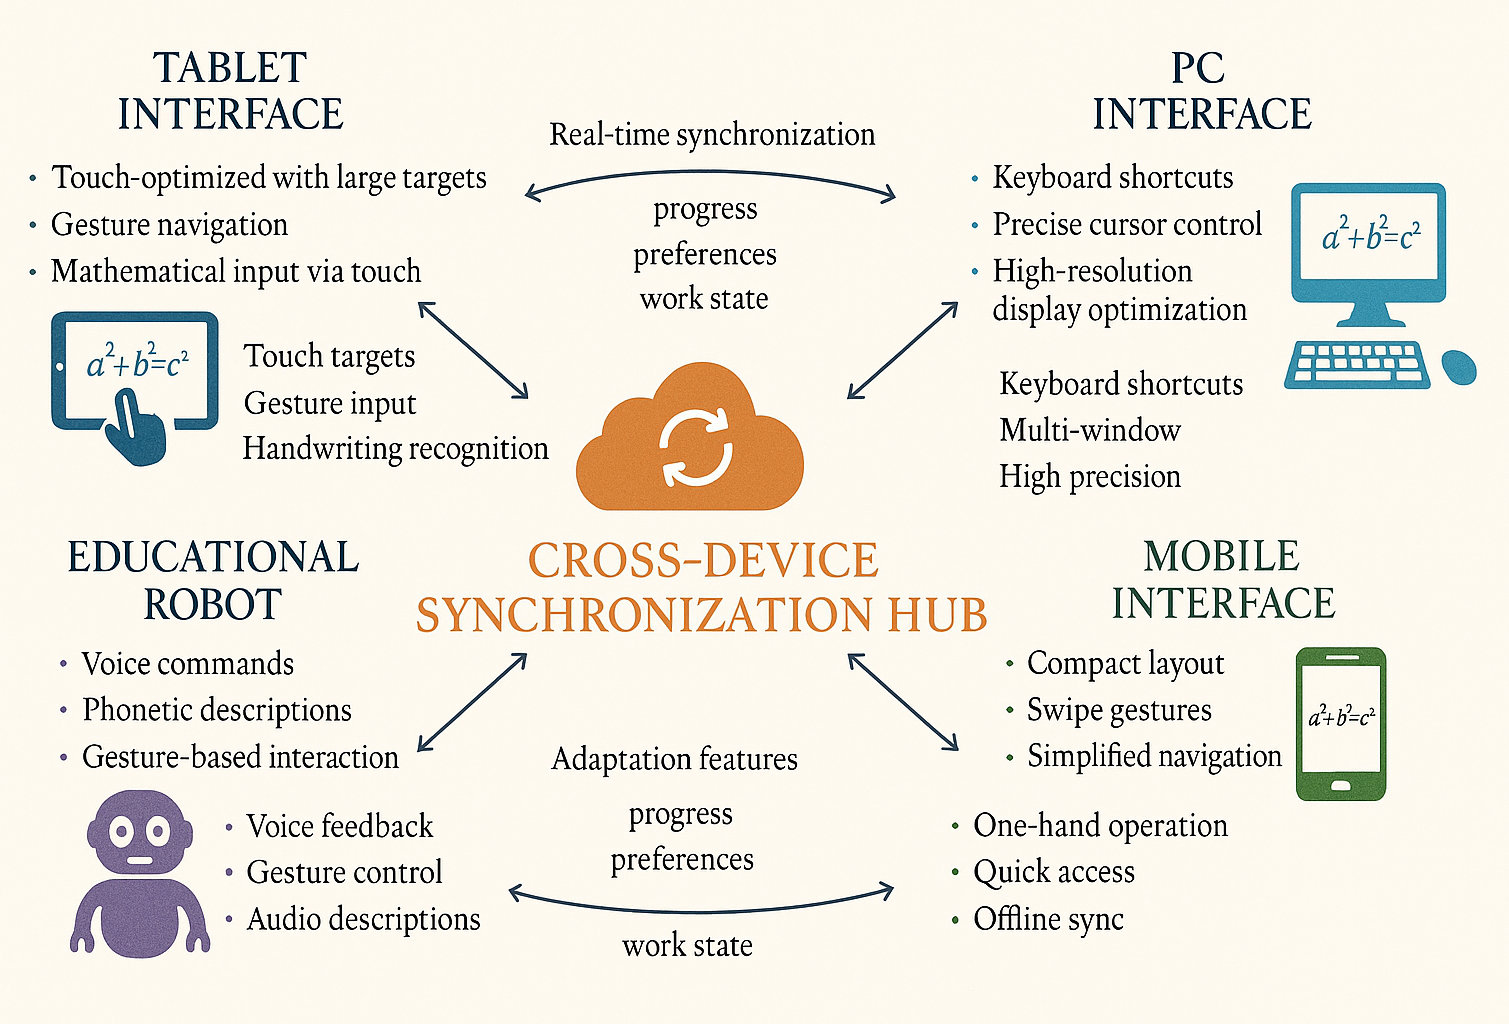
\includegraphics[width=\columnwidth]{4.png}}
\caption{Student Behavior Modeling Data Flow showing how learning interactions are analyzed to generate ALP profile data and LEG trajectory data, with examples of behavioral pattern recognition and temporal learning node creation.}
\label{fig:behavior_modeling}
\end{figure}

Problem difficulty is dynamically adjusted based on multiple factors that reflect the student's current learning state and progress. These factors include the student's recent performance trends to ensure appropriate challenge levels, time spent on similar problems to identify areas of difficulty, error frequency and types to understand specific challenges, and student confidence and engagement levels to maintain motivation and prevent frustration. This adaptive adjustment ensures that students are consistently challenged at an appropriate level that promotes learning without causing disengagement.

Each student receives a customized learning trajectory that addresses their unique needs and learning characteristics. This personalized approach addresses identified knowledge gaps by providing targeted remediation, builds on existing strengths to boost confidence and engagement, maintains optimal challenge levels to promote growth, and adapts to individual learning pace and preferences to ensure maximum effectiveness. The result is a learning experience that feels personally tailored to each student's needs and abilities.

\section{Dual-Value System Demonstration}

This section demonstrates how the connection mechanisms operate in practice through a comprehensive homework completion scenario that illustrates the simultaneous generation of personalized learning benefits and educational management insights. The demonstration shows how routine homework activities are transformed into rich data generation processes that serve both individual learning optimization and systematic educational oversight.

\subsection{Complete Homework Workflow Demonstration}

To illustrate how connection mechanisms generate dual value throughout the homework process, we present a comprehensive workflow example centered around a quadratic equations assignment that demonstrates the simultaneous enhancement of individual learning and generation of educational management data.

\textbf{Scenario}: A student named Alex receives a set of quadratic equation assignments through the polymorphic homework system, demonstrating how connection mechanisms generate dual value throughout the complete homework workflow.

\textbf{Initial Assignment Access}: When Alex logs into the homework system and selects the quadratic equations assignment, the system immediately begins generating dual-value data. The ALP framework captures Alex's login patterns, device preferences, and assignment selection behaviors to update personalized learning preferences while contributing to aggregate usage analytics that inform system optimization and resource allocation decisions. The LEG framework records this interaction as a new learning session node, connecting it to Alex's previous algebra learning trajectory while contributing to class-wide learning progression analytics.

\textbf{Problem-Solving Process}: As Alex begins solving quadratic equations, each interaction generates both immediate personalized support and systematic educational data. When Alex types mathematical expressions, the ALP-driven symbol recommendation system provides contextually appropriate symbol suggestions based on Alex's historical usage patterns and current problem context. Simultaneously, these interactions contribute to aggregate symbol usage analytics that inform curriculum design and instructional methodology decisions. The LEG framework tracks Alex's problem-solving strategy evolution, providing personalized difficulty adjustments while generating learning progression data that supports educational planning and intervention strategies.

\textbf{Help-Seeking and Support}: When Alex encounters difficulty with a particular quadratic equation type, the system's connection mechanisms demonstrate their dual-value generation capabilities. The knowledge point recommendation system provides immediate personalized assistance based on Alex's ALP profile and LEG learning trajectory, suggesting relevant concepts and problem-solving strategies tailored to Alex's learning preferences. Simultaneously, this help-seeking behavior contributes to systematic analytics that identify common difficulty points in quadratic equations, informing instructional design improvements and curriculum optimization decisions.

\textbf{Assignment Completion and Assessment}: Upon completing the assignment, Alex's submission triggers comprehensive dual-value generation processes. The system provides immediate personalized feedback and performance assessment based on Alex's individual learning profile and trajectory, while simultaneously contributing Alex's performance data to aggregate analytics that support classroom-level educational management decisions. The ALP framework updates Alex's knowledge mastery mapping and learning pathway recommendations, while the LEG framework records this completion as a significant learning milestone that informs future learning predictions and intervention planning.

\subsection{Dual-Value Output Analysis}

The homework completion scenario demonstrates how connection mechanisms generate comprehensive dual-value outputs that serve both individual learning enhancement and educational management functions. The individual learning benefits include personalized symbol recommendations that improve input efficiency, adaptive difficulty adjustments that maintain optimal challenge levels, targeted knowledge point suggestions that address specific learning gaps, and customized learning pathway updates that guide future study activities.

Simultaneously, the same homework activities generate systematic educational management insights including aggregate learning analytics that reveal class-wide learning patterns and trends, curriculum effectiveness data that inform instructional design improvements, intervention planning information that support proactive educational support strategies, and resource allocation guidance that optimize educational technology deployment. This dual-value generation demonstrates how connection mechanisms transform routine homework activities into comprehensive data generation processes that benefit all stakeholders in the educational ecosystem.



\textbf{Scenario}: A student receives a set of algebra assignments on a tablet device, requiring the input of complex mathematical expressions.

\begin{figure}[htbp]
\centerline{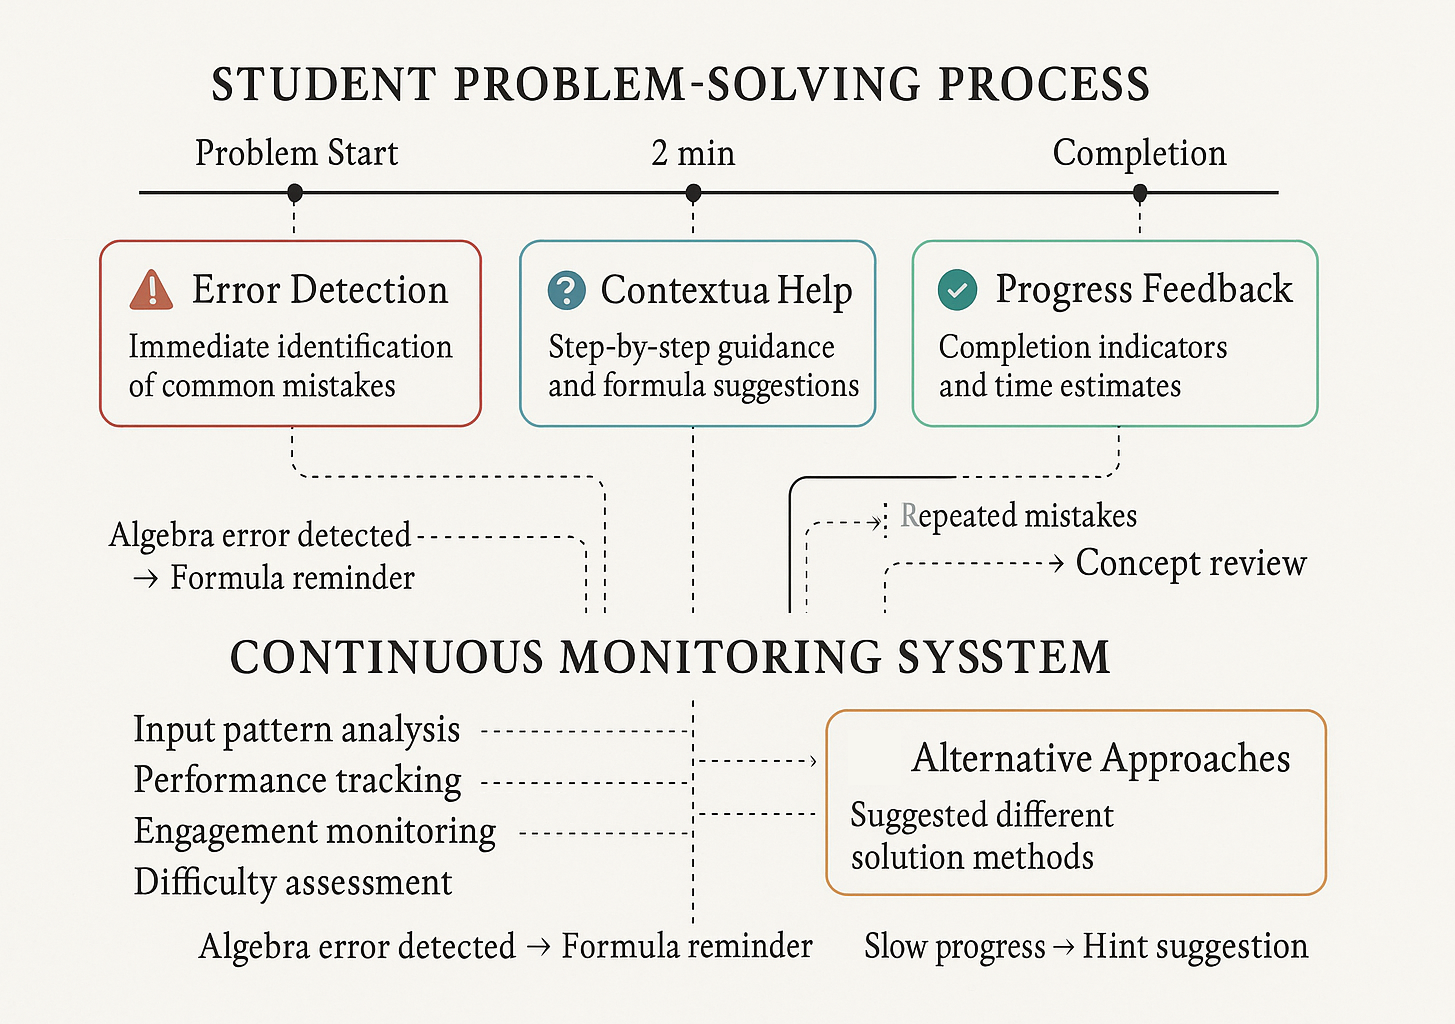
\includegraphics[width=\columnwidth]{5.png}}
\caption{Desktop Interface Implementation showing the ALP-driven personalized symbol recommendation panel, LEG-powered knowledge point suggestions, and integrated homework management system demonstrating framework-to-module mapping in practice.}
\label{fig:desktop_interface}
\end{figure}

\begin{figure}[htbp]
\centerline{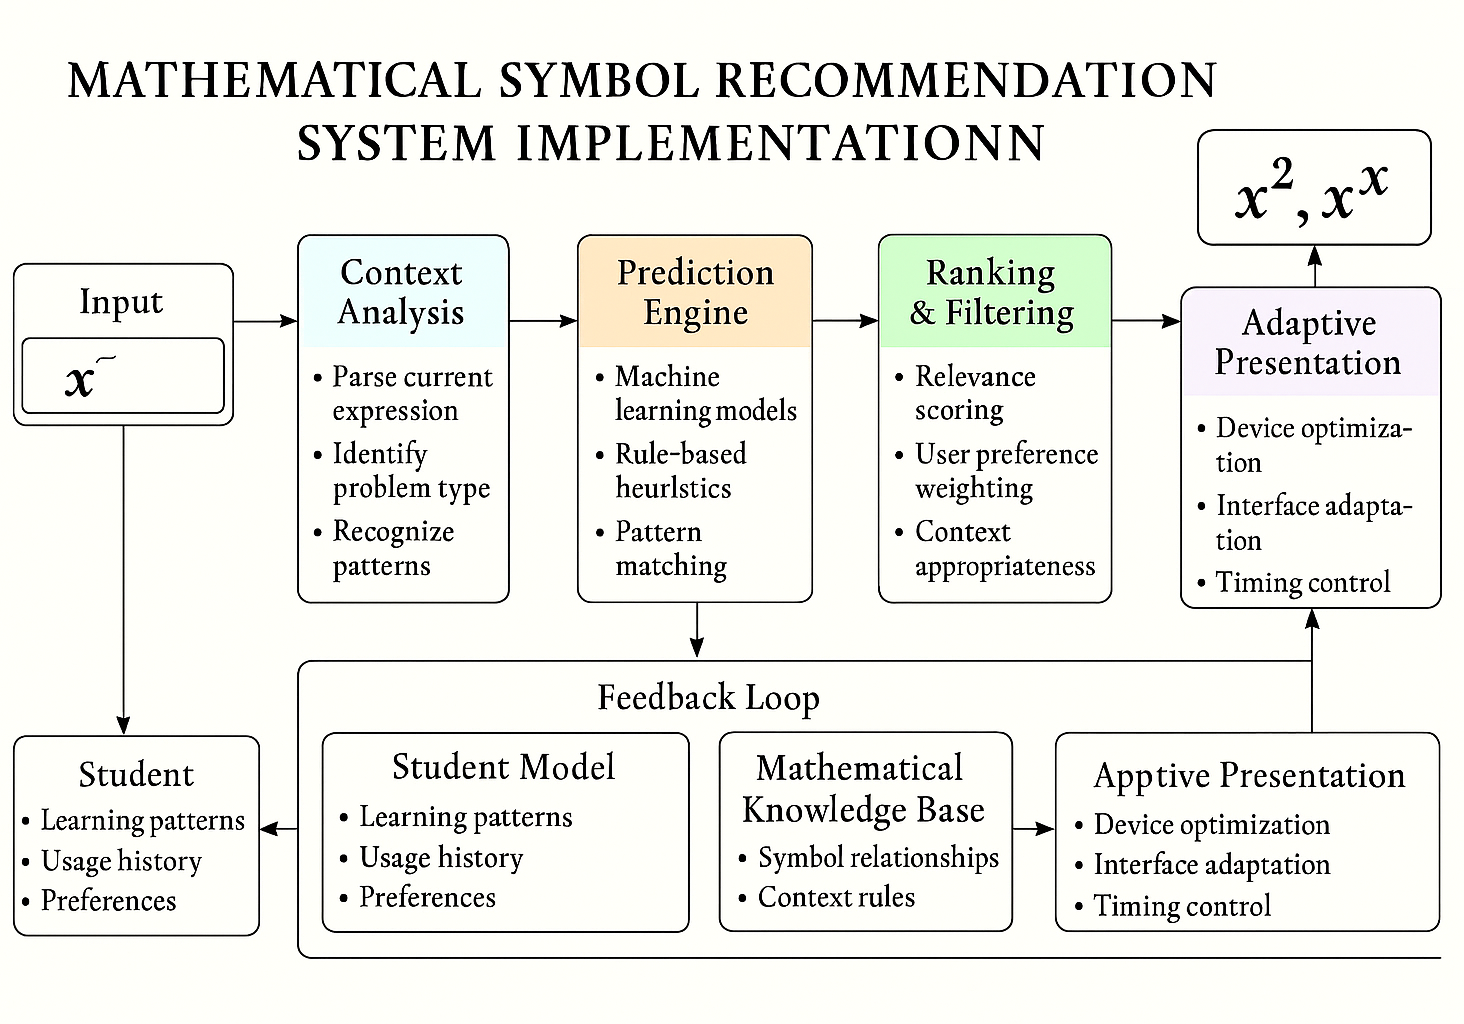
\includegraphics[width=\columnwidth]{6.png}}
\caption{Mobile Interface Implementation featuring responsive design adaptation with ALP-based personalized learning pathways and LEG-driven progress visualization, demonstrating cross-device framework consistency.}
\label{fig:mobile_interface}
\end{figure}



\begin{enumerate}
\item \textbf{Assignment Reception}: The student logs into the system, which automatically synchronizes assignments and creates personalized reminder schedules based on historical learning data and course progress.

\item \textbf{Intelligent Problem-Solving Assistance}: As the student begins inputting algebraic expressions, the Subject Symbol Dynamic Keyboard activates. For instance, when typing ``x\^{}'', the system immediately recommends commonly used exponent symbols such as ``$^2$'', ``$^3$'', and ``$^n$'', along with other potentially needed symbols.

\item \textbf{Knowledge Point Recommendation}: When students encounter difficulties, the system utilizes knowledge graph reasoning to recommend relevant algebraic formulas, theorems, or problem-solving strategies based on current solution steps and problem content.

\item \textbf{Solution Review and Instant Grading}: After completing a problem, students can request AI grading evaluation. The system instantly analyzes step-by-step solutions, providing immediate preliminary grading results with precise error location identification and corrective suggestions.

\item \textbf{Assignment Submission and Analysis}: Upon completion, the system performs final automated grading and generates detailed assignment reports including scores, error analysis, knowledge point mastery status, and personalized learning recommendations.
\end{enumerate}







\section{Conclusion and Future Work}

A comprehensive polymorphic homework system has been presented that demonstrates how connection mechanisms can simultaneously enhance personalized learning experiences and generate systematic educational management data. The system's innovative dual-support architecture proves that individual learning optimization and educational oversight are not competing objectives, but can be achieved synergistically through strategic connection point design and implementation.

The key contributions of this work include: (1) connection mechanism design that transforms routine homework activities into dual-value generation processes, (2) technical implementation strategies that embed connection points within existing homework system infrastructure without disrupting established workflows, (3) comprehensive demonstration of how ALP and LEG frameworks serve as connection bridges between personalized learning enhancement and educational management support, and (4) practical evidence that homework systems can serve as effective connection platforms that benefit all stakeholders in the educational ecosystem. The core innovation lies in proving that effective educational management does not require separate data collection systems or compromise student learning experiences, but can emerge naturally from well-designed connection mechanisms embedded within homework completion workflows.

This approach represents a fundamental shift from treating personalized learning and educational management as separate concerns to recognizing homework systems as natural connection platforms that can simultaneously optimize individual learning outcomes and support systematic educational oversight. The demonstrated connection mechanisms provide a practical framework for educational technology developers seeking to create systems that serve both student learning needs and institutional management requirements through unified, efficient, and effective design approaches.

The polymorphic design approach addresses fundamental limitations of traditional educational systems by providing adaptive, accessible, and personalized educational support. The system's ability to maintain consistent functionality while adapting to different devices and learning scenarios demonstrates how educational technology can be both powerful and flexible.

Future work includes expanding the knowledge graph services to cover additional mathematical domains, developing more sophisticated student behavior modeling algorithms, and investigating the integration of emerging technologies such as augmented reality for enhanced mathematical visualization. We also plan to explore the application of polymorphic design principles to other educational contexts beyond mathematics homework.



% 使用BibTeX管理参考文献
\bibliographystyle{IEEEtran}
\bibliography{IEEEabrv,references}

\end{document}
